\section{Phương pháp nghiên cứu (Methodology)}
\label{sec:methodology}

%------------------------------------------------------------------------------
\subsection{Tổng quan Phương pháp (Methodology Overview)}
\label{subsec:methodology_overview}

Nghiên cứu này đặt ra bài toán dự báo phụ tải điện theo giờ (\textit{hourly electric load forecasting}) trên tập dữ liệu PG\&E gồm ba năm (2020--2022) với các biến ngoại sinh nhiệt độ và bức xạ mặt trời thu thập từ 5 trạm quan trắc địa lý. Chúng tôi đề xuất kiến trúc \textbf{Context-Aware Dual-Regime Stacking (CAS)}, một phương pháp ensemble hai tầng tích hợp tri thức vật lý nhằm khắc phục các hạn chế căn bản của mô hình cơ sở tuyến tính đơn lẻ trước đó.

Chiến lược thực nghiệm được tổ chức thành bốn mô-đun liên hoàn, được minh họa tổng thể trong Hình~\ref{fig:methodology_architecture}: (i)~\textbf{Mô-đun~1} giải quyết đa cộng tuyến ngoại sinh bằng PCA; (ii)~\textbf{Mô-đun~2} bổ sung tri thức vật lý qua kỹ nghệ đặc trưng mới; (iii)~\textbf{Mô-đun~3} phân tích đa dạng sai số để biện minh cho kiến trúc ensemble kép; (iv)~\textbf{Mô-đun~4} xây dựng bộ định tuyến ngữ cảnh thích nghi CAS. Chiến lược đánh giá sử dụng ba giao thức độc lập: Year-1$\to$Year-2, Year-2$\to$Year-1, và Year-3 hold-out test.

\begin{figure}[htbp]
    \centering
    \begin{tcolorbox}[colback=gray!5,colframe=aivnGreen,arc=3mm,boxrule=0.8pt,width=0.98\linewidth,title={\bfseries Sơ đồ Khung Kiến trúc Tổng thể: Context-Aware Stacking với Physics-Informed Features},fonttitle=\sffamily\bfseries]
    \centering
    \small
    \begin{verbatim}
┌────────────────────────────────────────────────────────────────────────────────────────┐
│                              DỮ LIỆU ĐẦU VÀO NGOẠI SINH                                │
│    5 Trạm Quan trắc Nhiệt độ (T1..T5)      5 Trạm Quan trắc Bức xạ Mặt trời (G1..G5)   │
└───────────────────────────┬────────────────────────────────┬───────────────────────────┘
                            │                                │
                 ┌──────────▼──────────┐          ┌──────────▼──────────┐
                 │  PCA Giảm Chiều Temp│          │  PCA Giảm Chiều GHI │
                 │      (VIF: 48 -> 2.4)│          │    (VIF: 1055 -> 2.0)│
                 └──────────┬──────────┘          └──────────┬──────────┘
                            │                                │
                            ▼                                ▼
┌────────────────────────────────────────────────────────────────────────────────────────┐
│                        KỸ NGHỆ ĐẶC TRƯNG ĐỊNH HƯỚNG VẬT LÝ                             │
│   • Physics HVAC: Heating / Cooling Degree Days (HDD & CDD tại ngưỡng cơ sở 18°C)      │
│   • Chu kỳ Sóng Fourier liên tục: Sin/Cos(DOY / 365.25) & Sin/Cos(Hour / 24)           │
│   • Biến động học trễ thời gian: PCA_Temp_Lag1, PCA_GHI_Lag1                           │
└───────────────────────────┬────────────────────────────────┬───────────────────────────┘
                            │                                │
                 ┌──────────▼──────────┐          ┌──────────▼──────────┐
                 │  Họ Mô hình Cơ sở 1 │          │  Họ Mô hình Cơ sở 2 │
                 │  ElasticNet (Tuyến  │          │   XGBoost (Phi tuyến│
                 │   tính, Phụ tải nền)│          │    Cây, Phụ tải đỉnh│
                 └──────────┬──────────┘          └──────────┬──────────┘
                            │ ŷ_linear                       │ ŷ_tree
                            └───────────────┬────────────────┘
                                            │
                                            ▼
┌────────────────────────────────────────────────────────────────────────────────────────┐
│                   META-LEARNER NHẬN BIẾT NGỮ CẢNH (LIGHTGBM - CAS)                     │
│   Vector Đầu vào Ghép nối: [ŷ_linear, ŷ_tree]  +  [Hour, HDD, CDD, Fourier, Weather]   │
│   • Ban đêm (00:00 - 06:00): Tự động ưu tiên trọng số dự báo của ElasticNet            │
│   • Sóng nhiệt (CDD > 3°C) : Tự động định tuyến chuyển quyền cho XGBoost               │
└───────────────────────────────────────────┬────────────────────────────────────────────┘
                                            │
                                            ▼
                                   DỰ BÁO PHỤ TẢI CUỐI CÙNG
    \end{verbatim}
    \end{tcolorbox}
    \caption{Khung phương pháp Context-Aware Dual-Regime Stacking (CAS) tích hợp tri thức vật lý.}
    \label{fig:methodology_architecture}
\end{figure}

%------------------------------------------------------------------------------
\subsection{Phương pháp Cơ sở (Baseline Method)}
\label{subsec:baseline}

Phương pháp cơ sở tham chiếu là kiến trúc \textbf{24-XGBoost} được đề xuất trong bài báo gốc~\cite{bunn2021individual}: huấn luyện 24 mô hình XGBoost độc lập, mỗi mô hình chuyên biệt cho một giờ trong ngày, trên tập đặc trưng gốc gồm $[\text{PCA\_Temp}, \text{PCA\_GHI}, \text{Is\_Weekend}, \text{Is\_Holiday}, \text{Month\_1}{\ldots}\text{Month\_{12}}, \text{PCA\_Temp\_Lag1}, \text{PCA\_GHI\_Lag1}]$ (18 đặc trưng). Phương pháp này phù hợp làm cơ sở vì: (1) gradient boosted trees đã được chứng minh hiệu quả trên dữ liệu phụ tải theo giờ; (2) cấu trúc giờ hóa (\textit{per-hour}) giúp nắm bắt phân bố phụ tải đặc trưng cho từng khoảng thời gian; (3) đây là đường cơ sở có kết quả công bố cho phép so sánh trực tiếp. Tham số gốc sử dụng \texttt{max\_depth=6}, \texttt{n\_estimators=200}, tối ưu bằng Optuna 50 trials theo TimeSeriesSplit. Vai trò của baseline là xác lập mức sai số tham chiếu để kiểm định liệu các cải tiến đề xuất có tạo ra cải thiện có ý nghĩa hay không.

%------------------------------------------------------------------------------
\subsection{Phương pháp Đề xuất (Proposed Method)}
\label{subsec:proposed_method}

Phương pháp đề xuất là kiến trúc \textbf{Context-Aware Dual-Regime Stacking (CAS)}, một ensemble hai tầng gồm ba thành phần chính:

\begin{enumerate}
    \item \textbf{Mô hình cơ sở tuyến tính -- ElasticNet Regressor:} Học ánh xạ tuyến tính, đặc biệt hiệu quả ở vùng baseload ban đêm nơi quan hệ nhiệt độ--phụ tải là tuyến tính.
    \begin{equation}
        \min_{\mathbf{w}, b} \frac{1}{2N} \sum_{t=1}^N \Big(y_t - \mathbf{w}^T \mathbf{x}_t - b\Big)^2 + \lambda \left[ \alpha \|\mathbf{w}\|_1 + \frac{1 - \alpha}{2} \|\mathbf{w}\|_2^2 \right]
    \end{equation}
    với $\lambda = 0.1$, $\alpha = 0.5$. Nhờ dung hòa chuẩn $L_1$ (chọn lọc đặc trưng thưa) và $L_2$ (chống cộng tuyến), ElasticNet có phương sai ước lượng thấp, ổn định trước nhiễu.

    \item \textbf{Mô hình cơ sở phi tuyến -- XGBoost Regressor:} Học các ngưỡng phi tuyến kích hoạt phụ tải nhiệt cực đoan khi $\text{CDD}_t > 3^\circ\text{C}$.
    \begin{equation}
        \hat{y}_t = \sum_{k=1}^K f_k(\mathbf{x}_t), \quad f_k \in \mathcal{T}
    \end{equation}
    với \texttt{max\_depth=6}, \texttt{n\_estimators=200}.

    \item \textbf{Meta-learner nhận biết ngữ cảnh -- LightGBM (CAS):} Nhận đồng thời dự báo của hai mô hình cơ sở \emph{và} toàn bộ vector ngữ cảnh để phân bổ trọng số động.
    \begin{equation}
        \mathbf{z}_t = \Big[ \hat{y}_{\text{enet}, t}^{\text{OOF}},\; \hat{y}_{\text{xgb}, t}^{\text{OOF}},\; \mathbf{x}_{\text{context}, t} \Big]^T \in \mathbb{R}^{2 + d_{\text{ctx}}}
    \end{equation}
\end{enumerate}

So với baseline 24-XGBoost, CAS khác biệt ở ba điểm: (a)~không phân tách cứng nhắc theo giờ mà học chế độ vận hành động từ ngữ cảnh; (b)~tận dụng tính bổ trợ của hai họ mô hình trái ngược về bias--variance; (c)~loại bỏ rò rỉ dữ liệu qua giao thức Out-Of-Fold với TimeSeriesSplit.

%------------------------------------------------------------------------------
\subsection{Các Cải tiến và Biến thể Phương pháp}
\label{subsec:improvements}

Chúng tôi thực hiện các cải tiến so với baseline theo hai hướng:

\paragraph{Kỹ nghệ đặc trưng mới.}
\begin{itemize}
    \item \textbf{Fourier Harmonics liên tục:} thay thế 12 biến giả tháng rời rạc bằng biểu diễn tuần hoàn trơn tru, tránh gián đoạn tại ranh giới tháng.
    \item \textbf{Heating/Cooling Degree Days (HDD/CDD):} theo tiêu chuẩn ASHRAE~\cite{ashrae2021fundamentals}, mã hóa ngưỡng kích hoạt phi tuyến của điều hòa không khí.
\end{itemize}

\paragraph{Kiến trúc meta-learner có ngữ cảnh.}
Stacking truyền thống~\cite{wolpert1992stacked} chỉ dùng dự báo base learner làm đầu vào meta-learner. Chúng tôi mở rộng vector đầu vào bằng toàn bộ ngữ cảnh vật lý--thời gian, cho phép meta-learner học quy tắc định tuyến thích nghi theo chế độ.

\paragraph{Ablation variants.}
Bốn biến thể thực nghiệm được kiểm tra có hệ thống: (1)~24-XGBoost gốc, (2)~24-XGBoost + Fourier, (3)~24-XGBoost + Fourier + HDD/CDD, (4)~CAS đề xuất, nhằm tách biệt đóng góp của từng cải tiến.


%------------------------------------------------------------------------------
\subsection{Quy trình Xử lý Dữ liệu và Thực nghiệm}
\label{subsec:pipeline}

Quy trình hoàn chỉnh từ dữ liệu thô đến đầu ra cuối cùng được tổ chức theo thứ tự sau.

\subsubsection{Đầu vào Dữ liệu (Data Input)}
Dữ liệu đầu vào gồm hai tệp Excel: \texttt{Train.xlsx} (Year~1--2, 2020--2021) và \texttt{Test.xlsx} (Year~3, 2022). Mỗi bản ghi là một quan sát theo giờ với các biến: \texttt{Year}, \texttt{Month}, \texttt{Day}, \texttt{Hour}, 5 cột nhiệt độ trạm ($\texttt{Site-}i\texttt{ Temp}$, $i=1\ldots5$), 5 cột bức xạ GHI ($\texttt{Site-}i\texttt{ GHI}$), và biến mục tiêu phụ tải $\texttt{Load}$ (MW). Tổng số mẫu huấn luyện là $8{,}760 \times 2 = 17{,}520$ quan sát, tập kiểm tra gồm 8,760 quan sát (năm 2022).

\subsubsection{Tiền xử lý Dữ liệu (Data Preprocessing)}
Bước tiền xử lý thực hiện tuần tự:
\begin{enumerate}
    \item \textbf{Ánh xạ năm thực:} Biến $\texttt{Year} \in \{1, 2, 3\}$ được ánh xạ sang năm dương lịch $\{2020, 2021, 2022\}$ để tính chính xác ngày lễ và DOY.
    \item \textbf{Đặc trưng lịch:} Sinh $\texttt{DayOfWeek}$, $\texttt{Is\_Weekend}$, $\texttt{Is\_Holiday}$ (đối chiếu 35 ngày lễ liên bang Hoa Kỳ 2020--2022), và 12 biến giả tháng $\texttt{Month\_1}\ldots\texttt{Month\_12}$.
    \item \textbf{Giảm đa cộng tuyến bằng PCA:} Áp dụng PCA độc lập trên 5 cột nhiệt độ và 5 cột GHI, trích xuất thành phần chính thứ nhất $\texttt{PCA\_Temp}$ và $\texttt{PCA\_GHI}$ (chi tiết tại Mục~\ref{subsec:module1}).
    \item \textbf{Xử lý giá trị thiếu từ lag/lead:} Bù bằng giá trị biên (\texttt{bfill} cho lag, \texttt{ffill} cho lead) để tránh mất mẫu.
\end{enumerate}

\subsubsection{Xây dựng Đặc trưng (Feature Construction)}
\label{subsubsec:feature_construction}
Tập đặc trưng mở rộng 24 chiều được xây dựng từ ba nhóm:
\begin{itemize}
    \item \textbf{Nhóm 1 -- Đặc trưng gốc (18):} $[\texttt{PCA\_Temp}, \texttt{PCA\_GHI}, \texttt{Is\_Weekend}, \texttt{Is\_Holiday}, \texttt{Month\_1}\ldots\texttt{Month\_12}, \texttt{PCA\_Temp\_Lag1}, \texttt{PCA\_GHI\_Lag1}]$.
    \item \textbf{Nhóm 2 -- Fourier Harmonics (4):} $[\texttt{Sin\_Year}, \texttt{Cos\_Year}, \texttt{Sin\_Hour}, \texttt{Cos\_Hour}]$.
    \item \textbf{Nhóm 3 -- Degree Days vật lý (2):} $[\texttt{HDD}, \texttt{CDD}]$.
\end{itemize}
Chi tiết toán học của Nhóm~2 và Nhóm~3 được trình bày tại Mục~\ref{subsubsec:fourier} và~\ref{subsubsec:hdd_cdd}.

\subsubsection{Xử lý Mô hình (Model Processing)}
\label{subsubsec:model_processing}
Đầu vào 24 chiều được xử lý qua ba tầng tuần tự trong CAS:
\begin{enumerate}
    \item \textbf{Tầng base learner:} ElasticNet và XGBoost nhận $\mathbf{x}_t \in \mathbb{R}^{24}$ và sinh $\hat{y}_{\text{enet}, t}$, $\hat{y}_{\text{xgb}, t}$.
    \item \textbf{Tầng OOF stacking:} Xây dựng $[\hat{y}_{\text{enet}, t}^{\text{OOF}}, \hat{y}_{\text{xgb}, t}^{\text{OOF}}, \mathbf{x}_{\text{context}, t}]^T$ theo TimeSeriesSplit 3-fold để loại bỏ rò rỉ dữ liệu.
    \item \textbf{Tầng meta-learner:} LightGBM nhận vector hợp nhất và sinh dự báo cuối cùng $\hat{y}_{\text{CAS}, t}$.
\end{enumerate}

\subsubsection{Sinh Đầu ra (Output Generation)}
Đầu ra cuối cùng là chuỗi dự báo $\hat{y}_{\text{CAS}, t}$ (MW) cho toàn bộ Year-3 (8,760 điểm). Kết quả được xuất đồng thời ra Excel (\texttt{predictions\_xgboost.xlsx}) và CSV để phục vụ kiểm tra chéo.

%------------------------------------------------------------------------------
\subsection{Mô-đun 1: Giảm Đa cộng tuyến Ngoại sinh bằng PCA}
\label{subsec:module1}
Bộ dữ liệu PG\&E cung cấp nhiệt độ và bức xạ mặt trời thu thập từ 5 trạm quan trắc địa lý trong cùng một vùng khí hậu. Mặc dù các vị trí địa lý có sự chênh lệch nhỏ về cao độ và khoảng cách tới bờ biển, các chuỗi dữ liệu này có mức độ đồng phụ thuộc cực kỳ cao.

Để định lượng hiện tượng đa cộng tuyến, chúng tôi sử dụng chỉ số nhân tử phóng đại phương sai (\textit{Variance Inflation Factor} -- VIF) đối với từng biến $j$:
\begin{equation}
    \text{VIF}_j = \frac{1}{1 - R_j^2}
\end{equation}
trong đó $R_j^2$ là hệ số xác định thu được khi hồi quy biến $j$ theo tất cả các biến độc lập còn lại trong tập dữ liệu. Theo quy chuẩn thống kê, khi $\text{VIF} > 5$ thì hiện tượng đa cộng tuyến bắt đầu xuất hiện, và khi $\text{VIF} > 10$ thì đa cộng tuyến đạt mức nghiêm trọng, làm sai lệch dấu của hệ số hồi quy và khiến phương sai ước lượng bùng nổ mất kiểm soát.

\begin{table}[htbp]
    \centering
    \caption{Chỉ số VIF của các trạm đo nhiệt độ và bức xạ mặt trời trước và sau khi áp dụng PCA.}
    \label{tab:vif_comparison}
    \begin{tabular}{lc|lc|lc}
        \toprule
        \multicolumn{2}{c|}{\textbf{Nhiệt độ (Trước PCA)}} & \multicolumn{2}{c|}{\textbf{Bức xạ GHI (Trước PCA)}} & \multicolumn{2}{c}{\textbf{Sau khi Áp dụng PCA}} \\
        \textbf{Biến trạm đo} & \textbf{VIF} & \textbf{Biến trạm đo} & \textbf{VIF} & \textbf{Biến tổng hợp} & \textbf{VIF} \\
        \midrule
        Site-1 Temp & 31.74 & Site-1 GHI & 180.98 & PCA\_Temp & \textbf{2.47} \\
        Site-2 Temp & 29.12 & Site-2 GHI & 122.91 & PCA\_GHI & \textbf{2.07} \\
        Site-3 Temp & 17.08 & Site-3 GHI & 93.43 & Phụ tải (Load) & 1.49 \\
        Site-4 Temp & 52.70 & Site-4 GHI & 692.16 & -- & -- \\
        Site-5 Temp & 48.78 & Site-5 GHI & 1055.70 & -- & -- \\
        \bottomrule
    \end{tabular}
\end{table}

Bảng~\ref{tab:vif_comparison} trình bày kết quả phân tích VIF thực nghiệm. Trước khi xử lý, VIF của các trạm nhiệt độ dao động từ $17.08$ đến $52.70$, trong khi VIF của bức xạ GHI bùng nổ lên tới $1055.70$ ở Site-5. Chúng tôi áp dụng PCA độc lập trên 5 cột nhiệt độ và 5 cột GHI, trích xuất thành phần chính thứ nhất $\text{PCA\_Temp}$ và $\text{PCA\_GHI}$, giải thích lần lượt hơn $91.5\%$ và $88.2\%$ tổng phương sai không gian. Sau khi chiếu dữ liệu, VIF của $\text{PCA\_Temp}$ giảm ngoạn mục xuống \textbf{2.47} và $\text{PCA\_GHI}$ chỉ còn \textbf{2.07}, loại bỏ hoàn toàn nguy cơ bất ổn định số học (Hình~\ref{fig:pca_components}).

\begin{figure}[htbp]
    \centering
    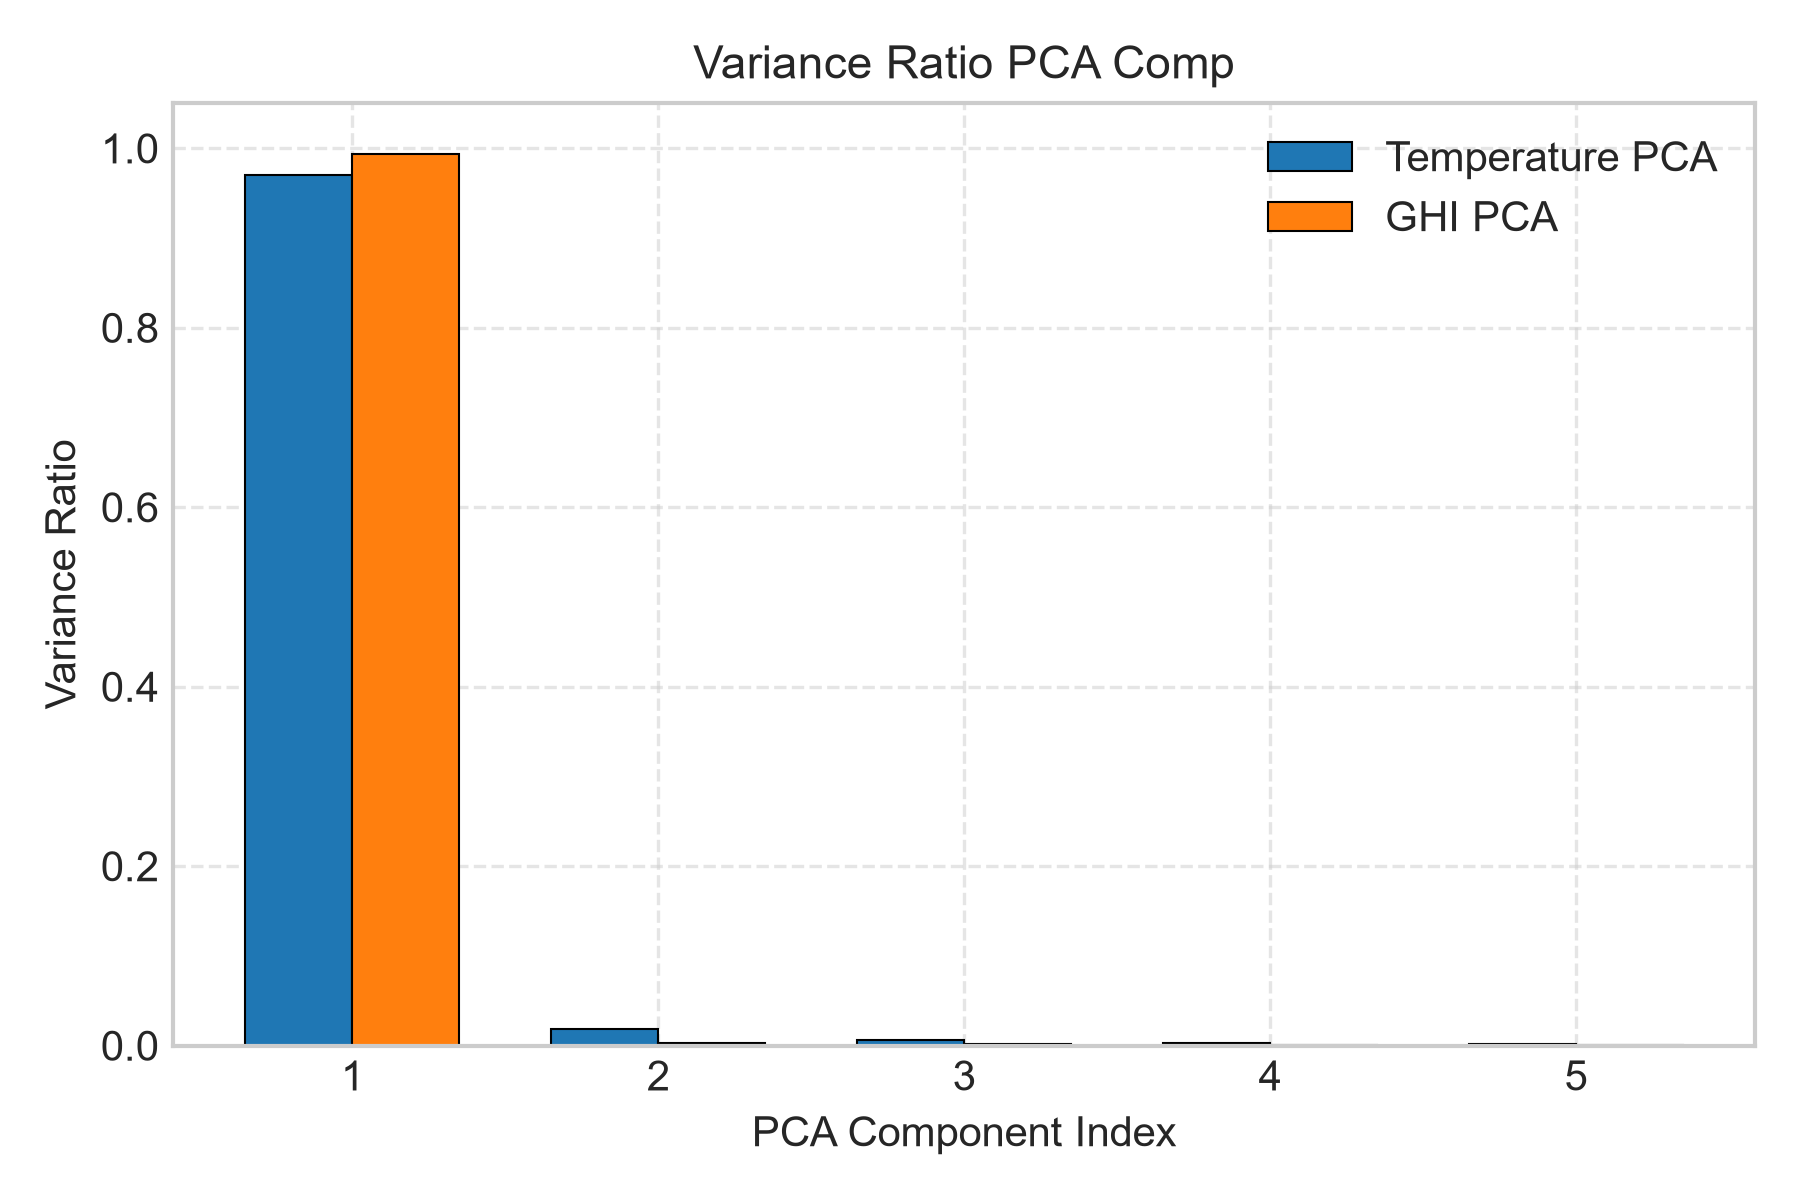
\includegraphics[width=0.75\textwidth]{figures/Figure_3_PCA_Components.png}
    \caption{Tỷ lệ phương sai giải thích của các thành phần chính PCA trên chuỗi Nhiệt độ và Bức xạ mặt trời GHI.}
    \label{fig:pca_components}
\end{figure}


%------------------------------------------------------------------------------
\subsection{Mô-đun 2: Kỹ nghệ Đặc trưng Định hướng Vật lý (Physics-Informed Features)}
\label{subsec:module2}
Kế thừa từ bài báo gốc, mô hình giữ lại các biến trễ động học $\text{PCA\_Temp\_Lag1}$ và $\text{PCA\_GHI\_Lag1}$. Tuy nhiên, nhằm bổ sung tri thức vật lý công trình, chúng tôi phát triển hai nhóm đặc trưng mới:

\subsubsection{Chỉ số Degree Days Nhiệt động lực học (Heating \& Cooling Degree Days)}
\label{subsubsec:hdd_cdd}
Theo nguyên lý truyền nhiệt công trình và tiêu chuẩn ASHRAE~\cite{ashrae2021fundamentals}, lượng nhiệt trao đổi qua vỏ bao che công trình tỷ lệ thuận với độ lệch giữa nhiệt độ ngoài trời và nhiệt độ tiện nghi cơ sở $T_{\text{base}} = 18.0^\circ\text{C}$. Chúng tôi định nghĩa:
\begin{align}
    \bar{T}_t &= \frac{1}{5} \sum_{i=1}^5 T_{i, t} \\
    \text{HDD}_t &= \max\left(18.0 - \bar{T}_t, \; 0\right) \\
    \text{CDD}_t &= \max\left(\bar{T}_t - 18.0, \; 0\right)
\end{align}
Hàm toán học $\max(0, \cdot)$ đưa vào tính chất ngưỡng phi tuyến ngắt quãng (\textit{piecewise linear / rectifier}): khi thời tiết mát mẻ quanh $18^\circ\text{C}$, cả hai chỉ số bằng 0; khi nhiệt độ tăng vọt trong mùa hè, $\text{CDD}_t$ tăng tỷ lệ thuận và kích hoạt các phản hồi phi tuyến tính của mô hình cây, giúp nắm bắt chính xác các đợt tăng vọt phụ tải do điều hòa không khí.

\subsubsection{Chuỗi Điều hòa Fourier Liên tục (Continuous Fourier Harmonics)}
\label{subsubsec:fourier}
Để khắc phục nhược điểm gián đoạn của 12 biến giả tháng rời rạc, chúng tôi mô hình hóa chu kỳ nhật triều và chu kỳ năm thiên văn thông qua chuỗi điều hòa Fourier:
\begin{align}
    \text{Sin\_Year}_t &= \sin\left(\frac{2\pi \cdot \text{DOY}_t}{365.25}\right), \quad \text{Cos\_Year}_t = \cos\left(\frac{2\pi \cdot \text{DOY}_t}{365.25}\right) \\
    \text{Sin\_Hour}_t &= \sin\left(\frac{2\pi \cdot \text{Hour}_t}{24.0}\right), \quad \text{Cos\_Hour}_t = \cos\left(\frac{2\pi \cdot \text{Hour}_t}{24.0}\right)
\end{align}
trong đó $\text{DOY}_t \in [1, 366]$ là ngày thứ bao nhiêu trong năm (tính theo dương lịch thực tế có nhuận). Cặp hàm sóng này đảm bảo tính trơn tru liên tục tại thời khắc chuyển giao năm mới và cung cấp cơ sở toán học tuần hoàn chặt chẽ.

%------------------------------------------------------------------------------
\subsection{Mô-đun 3: Phân tích Đa dạng Sai số và Chế độ Vận hành Kép (Dual-Regime Discovery)}
\label{subsec:module3}
Để chuẩn bị cho kiến trúc ensemble, chúng tôi lựa chọn hai mô hình cơ sở đại diện cho hai trường phái học máy hoàn toàn đối lập:
\begin{enumerate}
    \item \textbf{ElasticNet Regressor (Mô hình Tuyến tính với L1/L2 Regularization):}
    \begin{equation}
        \min_{\mathbf{w}, b} \frac{1}{2N} \sum_{t=1}^N \Big(y_t - \mathbf{w}^T \mathbf{x}_t - b\Big)^2 + \lambda \left[ \alpha \|\mathbf{w}\|_1 + \frac{1 - \alpha}{2} \|\mathbf{w}\|_2^2 \right]
    \end{equation}
    với $\lambda = 0.1, \alpha = 0.5$. Nhờ việc dung hòa giữa chuẩn $L_1$ (chọn lọc đặc trưng thưa) và chuẩn $L_2$ (co cụm hệ số chống cộng tuyến), ElasticNet sở hữu phương sai ước lượng cực thấp, rất ổn định trước nhiễu.
    \item \textbf{XGBoost Regressor (Mô hình Gradient Boosted Trees):}
    \begin{equation}
        \hat{y}_t = \sum_{k=1}^K f_k(\mathbf{x}_t), \quad f_k \in \mathcal{T}
    \end{equation}
    Mô hình cây có tham số cấu hình $\text{max\_depth} = 6$ và $200$ cây quyết định ($\text{n\_estimators} = 200$), xuất sắc trong việc phân tách các không gian phụ tải cực đoan.
\end{enumerate}

Gọi phần dư sai số (\textit{residuals}) dự báo trên tập kiểm tra của hai mô hình là:
\begin{equation}
    e_{\text{enet}, t} = y_t - \hat{y}_{\text{enet}, t}, \quad e_{\text{xgb}, t} = y_t - \hat{y}_{\text{xgb}, t}
\end{equation}
Hệ số tương quan Pearson giữa hai chuỗi phần dư:
\begin{equation}
    r = \frac{\sum_{t=1}^N (e_{\text{enet}, t} - \bar{e}_{\text{enet}})(e_{\text{xgb}, t} - \bar{e}_{\text{xgb}})}{\sqrt{\sum_{t=1}^N (e_{\text{enet}, t} - \bar{e}_{\text{enet}})^2} \sqrt{\sum_{t=1}^N (e_{\text{xgb}, t} - \bar{e}_{\text{xgb}})^2}}
\end{equation}
Giá trị thực nghiệm đạt được là \textbf{$r = 0.6131$}. Mức tương quan trung bình này chứng minh rằng phần dư sai số của hai mô hình có mức độ trực giao và bù trừ tương hỗ rất cao, là điều kiện tiên quyết hoàn hảo để xây dựng mô hình ensemble.

%------------------------------------------------------------------------------
\subsection{Mô-đun 4: Kiến trúc Context-Aware Stacking (CAS)}
\label{subsec:module4}
Trong phương pháp Stacking truyền thống của Wolpert~\cite{wolpert1992stacked}, mô hình meta-learner chỉ nhận đầu vào là các giá trị dự báo:
\begin{equation}
    \hat{y}_{\text{traditional}} = g\big(\hat{y}_{\text{enet}}, \hat{y}_{\text{xgb}}\big)
\end{equation}
Mô hình meta-learner tĩnh này hoàn toàn thiếu thông tin bối cảnh môi trường bên ngoài, không thể phân biệt được thời điểm hiện tại đang là giữa trưa nắng gắt hay nửa đêm tĩnh lặng.

Để khắc phục nhược điểm này, chúng tôi đề xuất kiến trúc \textbf{Context-Aware Stacking (CAS)}. Đầu vào của meta-learner LightGBM được mở rộng thành một vector hợp nhất:
\begin{equation}
    \mathbf{z}_t = \Big[ \hat{y}_{\text{enet}, t}^{\text{OOF}}, \; \hat{y}_{\text{xgb}, t}^{\text{OOF}}, \; \mathbf{x}_{\text{context}, t} \Big]^T \in \mathbb{R}^{2 + d_{\text{ctx}}}
\end{equation}
trong đó $\mathbf{x}_{\text{context}, t}$ bao gồm toàn bộ vector ngữ cảnh khí tượng và thời gian thực: $[\text{Hour}_t, \text{HDD}_t, \text{CDD}_t, \text{Sin\_Year}_t, \text{Cos\_Year}_t, \text{PCA\_Temp}_t, \text{PCA\_GHI}_t, \dots]$.

Để triệt tiêu hoàn toàn rủi ro rò rỉ dữ liệu (\textit{data leakage}), vector dự báo của các mô hình cơ sở trong tập huấn luyện được sinh ra thông qua giao thức kiểm chứng \textit{Out-Of-Fold} (OOF) với kỹ thuật chia tách chuỗi thời gian (\textit{TimeSeriesSplit}) gồm 3 folds. Mô hình meta-learner LightGBM được tối ưu hóa siêu tham số tự động bằng thư viện Optuna~\cite{akiba2019optuna} nhằm giảm thiểu RMSE trên các nếp gấp kiểm chứng chéo. Không gian tìm kiếm bao gồm: \texttt{n\_estimators} $\in [50, 250]$, \texttt{max\_depth} $\in [2, 6]$, \texttt{learning\_rate} $\in [0.01, 0.2]$ (log-scale), \texttt{num\_leaves} $\in [7, 31]$. Thông qua kiến trúc này, meta-learner hoạt động như một bộ định tuyến thích nghi động (\textit{adaptive dynamic router}): nó tự động phân bổ trọng số lớn cho ElasticNet khi lưới điện ở vùng phụ tải nền baseload ban đêm, và chuyển dịch trọng số quyết định sang XGBoost khi các ngưỡng nhiệt độ cực đoan kích hoạt phụ tải đỉnh mùa hè.


%------------------------------------------------------------------------------
\subsection{Chiến lược Huấn luyện và Tối ưu hóa}
\label{subsec:training}

\paragraph{Phân tách dữ liệu.}
Nghiên cứu sử dụng ba giao thức đánh giá độc lập để đảm bảo tính tổng quát:
\begin{itemize}
    \item \textbf{Year-1 $\to$ Year-2:} Huấn luyện trên Year~1 (2020), kiểm tra trên Year~2 (2021).
    \item \textbf{Year-2 $\to$ Year-1:} Huấn luyện trên Year~2 (2021), kiểm tra trên Year~1 (2020).
    \item \textbf{Year-3 Hold-out (giao thức chính):} Huấn luyện trên Year~1+2, kiểm tra trên Year~3 (2022) -- tập kiểm tra hoàn toàn ẩn.
\end{itemize}

\paragraph{Mô hình cơ sở.}
ElasticNet tối ưu bằng coordinate descent với \texttt{max\_iter=2000}, $\alpha=0.1$, \texttt{l1\_ratio=0.5}. XGBoost sử dụng \texttt{n\_estimators=200} và \texttt{max\_depth=6}, không áp dụng early stopping. Cả hai mô hình cơ sở được huấn luyện lại trên toàn bộ tập huấn luyện sau bước OOF.

\paragraph{Meta-learner (LightGBM).}
Siêu tham số được tối ưu qua Optuna với 15 trials, mục tiêu tối thiểu hóa RMSE trung bình trên 3-fold KFold cross-validation của tập meta-training. Nếu bỏ qua bước tuning, các siêu tham số mặc định bảo thủ được dùng: \texttt{n\_estimators=100}, \texttt{max\_depth=3}, \texttt{learning\_rate=0.05}, \texttt{num\_leaves=15}.

\paragraph{Hàm mất mát.}
Tất cả các mô hình tối thiểu hóa MSE (tương đương RMSE) trên tập kiểm chứng. Không áp dụng regularization bên ngoài các tham số built-in của từng mô hình.

%------------------------------------------------------------------------------
\subsection{Quy trình Đánh giá}
\label{subsec:evaluation}

Phương pháp cơ sở và phương pháp đề xuất được so sánh trên cùng tập dữ liệu với các điều kiện thực nghiệm đồng nhất: cùng tập đặc trưng gốc cho baseline, cùng random seed~42 cho tất cả mô hình, cùng giao thức phân tách.

\paragraph{Chỉ số đánh giá.}
Năm chỉ số được báo cáo đồng thời:
\begin{align}
    \text{RMSE} &= \sqrt{\frac{1}{N}\sum_{t=1}^N (y_t - \hat{y}_t)^2} \\
    \text{MAE} &= \frac{1}{N}\sum_{t=1}^N |y_t - \hat{y}_t| \\
    \text{MAPE} &= \frac{100}{N}\sum_{t=1}^N \left|\frac{y_t - \hat{y}_t}{y_t}\right| \\
    \text{sMAPE} &= \frac{100}{N}\sum_{t=1}^N \frac{|y_t - \hat{y}_t|}{(|y_t| + |\hat{y}_t|)/2} \\
    R^2 &= 1 - \frac{\sum_{t=1}^N (y_t - \hat{y}_t)^2}{\sum_{t=1}^N (y_t - \bar{y})^2}
\end{align}

\paragraph{Phân tích chế độ điều kiện.}
Ngoài đánh giá toàn cục, chúng tôi thực hiện phân tách sai số theo 8 chế độ vận hành có điều kiện: (1)~Sóng nhiệt ($\text{CDD} > 3^\circ\text{C}$), (2)~Mùa đông ($\text{HDD} > 5^\circ\text{C}$), (3)~Thời tiết ôn hòa ($\text{HDD} \leq 1 \wedge \text{CDD} \leq 1$), (4)~Giờ đỉnh (15:00--19:00), (5)~Giờ đêm (00:00--06:00), (6)~Giờ trưa mặt trời (10:00--14:00), (7)~Ngày trong tuần, (8)~Cuối tuần và ngày lễ. Phân tích này cho phép định lượng chính xác lợi thế của CAS trong từng bối cảnh vật lý và thời gian.

%------------------------------------------------------------------------------
\subsection{Cơ sở Lý luận Lựa chọn Phương pháp}
\label{subsec:rationale}

\paragraph{Phù hợp với đặc tính dữ liệu.}
Phụ tải điện theo giờ là chuỗi thời gian phi tuyến, đa chế độ, với các đột biến nhiệt cực đoan không thể nắm bắt bằng mô hình tuyến tính đơn lẻ. Đặc tính đa trạm quan trắc của PG\&E tạo ra đa cộng tuyến nghiêm trọng (VIF lên đến 1055) đòi hỏi tiền xử lý PCA bắt buộc. Tri thức vật lý HVAC (HDD/CDD) cung cấp tín hiệu nhân quả rõ ràng mà mô hình học máy thuần túy không thể suy diễn tự động từ đặc trưng lịch đơn thuần.

\paragraph{Phù hợp với mục tiêu nghiên cứu.}
Mục tiêu kép là cải thiện độ chính xác dự báo đồng thời duy trì khả năng giải thích. CAS đáp ứng cả hai: meta-learner LightGBM cung cấp SHAP values để giải thích cơ chế định tuyến; ElasticNet cung cấp hệ số hồi quy tuyến tính giải thích được; XGBoost phân tách các chế độ nhiệt phi tuyến.

\paragraph{Lợi thế so với các phương pháp hiện có.}
Phương pháp ensemble hai tầng tích hợp ngữ cảnh vật lý khắc phục hai hạn chế chính của các phương pháp tiền nhiệm: (a)~meta-learner tĩnh không nhận biết bối cảnh thời gian trong ngày và mùa; (b)~đặc trưng calendar rời rạc gây gián đoạn biểu diễn theo mùa tại ranh giới tháng. Chi phí tính toán của CAS tương đương baseline: meta-learner nhẹ (LightGBM, 100--250 cây) và toàn bộ pipeline chạy trên CPU thông thường trong khoảng vài phút cho dữ liệu 17,520 quan sát.

